% Täällä kerrotaan aikaisemmista, vastaavista projekteista

\section{Aikaisempia opetuskieliä}
Ohjelmoinnin opetukseen on kehitelty
monia erilaisia ohjelmointikieliä.
Tässä luvussa esitellään muutamia
historiallisesti merkittäviä
kieliä ohjelmoinnin aloitukseen.
Lisäksi esitellään myös muutamia uusia
ohjelmointikieliä, jotka toimivat
EppaBasicin tavoin selainympäristössä.

Yksi ensimmäisistä ohjelmoinnin
opetukseen kehitetyistä
ohjelmointikielistä oli
Dartmouth Collegessa vuonna 1964
kehitetty BASIC \cite{basic}.
BASIC kehitettiin erityisesti
opiskelijoille, joilla ei ollut
tietojenkäsittelytieteellistä
taustaa \cite{language_history}.
Alkuperäinen Basic oli hyvin
rajoittunut, mutta myöhemmät
murteet ovat tuoneet mukanaan
kieleen uusia ominaisuuksia.

Basicista on tehty
monia muunnoksia, murteita.
Yksi merkittävimmistä
Basic-murteista on
Microsoftin kehittämä
Visual Basic \cite{vb.net}.
Microsoft on kehittänyt myös
lapsille tarkoitetun kielen
Small Basic \cite{sb}.
Pelien kehittämiseen on suunniteltu
esimerkiksi Blitz Researchin
Blitz Basic \cite{bb}.
Toisaalta myös suomalaisen
Jukka Lavosen kehittämä
CoolBasic \cite{cb} on ollut merkittävä
EppaBasicin kannalta, sillä
se on inspiroinut EppaBasicin
kehitystyötä.

Ohjelmointikielet, jotka ovat
toistensa murteita,
muistuttavat rakenteeltaan
toisiaan.
Murteet eivät välttämättä
ole yhteensopivia keskenään,
joten niitä voidaan kutsua
myös omiksi kielikseen.
Tästä syystä murteilla
usein onkin omat nimensä.

Yksi ensimmäisistä ohjelmointikielistä,
jolla pystyi tekemään grafiikkaa,
oli vuonna 1967 kehitetty Logo.
Se muistetaan erityisesti
kilpikonna-grafiikastaan,
jossa ohjelmakomennoilla
siirretään kilpikonnaa,
joka piirtää kulkiessaan
näytölle viivan.
Logo on saanut vaikutteita vuonna 1958
julkaistusta Lisp-ohjelmointikielestä.

Vuonna 1970 Niklaus Wirth
julkaisi Pascal-ohjelmointikielen
\cite{pascal}.
Kieli suunniteltiin erityisesti
opetuskäyttöön, ja se yhdisti
aikansa yleisimpien ohjelmointikielten
parhaiksi katsottuja ominaisuuksia
\cite{language_history}.

Python \cite{python} on
Guido van Rossumin vuonna 1990
julkaisema ohjelmointikieli.
Nykyisin kieltä kehittää
Python Software Foundation.
Python on yleisesti käytössä ohjelmoinnin
opetuksessa ympäri maailmaa.
Esimerkiksi Aalto yliopistossa
ensimmäisiä ohjelmointikursseja
on opetettu Pythonilla.

Java \cite{java} on Sun Microsystemsin
vuonna 1995 julkaisema,
nykyisin Oraclen kehittämä
oliopohjainen ohjelmointikieli.
Myös ja on yleisesti käytössä
ohjelmoinnin opetuksessa.
Esimerkiksi Helsingin yliopiston
tietojenkäsittelytieteen ensimmäiset
kurssit opetetaan Javalla.

\fxnote{Rubysta jotain}

2000-luvulle tultaessa alkoi
verkkoselainten kehittyessä
ilmestyä ohjelmointikieliä
myös selainympäristöön.
Tällaisille kielille on tyypillistä,
että niillä voi helposti luoda
ainakin yksinkertaista grafiikkaa.

Eräs selainympäristössä toimiva
ohjelmointikieli on
MIT:n kehittämä
Scratch-ohjelmoin\-ti\-kieli
\cite{scratch}
(ks. Kuva \ref{img:scratch}).
Scratch on visuaalinen ohjelmointikieli,
mikä tarkoittaa sitä, että
kieltä ohjelmoidaan raahaamalla
hiirellä komentopalikoita
ohjelmointialueelle.
Komentopalikoiden avulla
voi liikuttaa ja pyörittää
kuvia.

\begin{figure}[h]
    \centering
    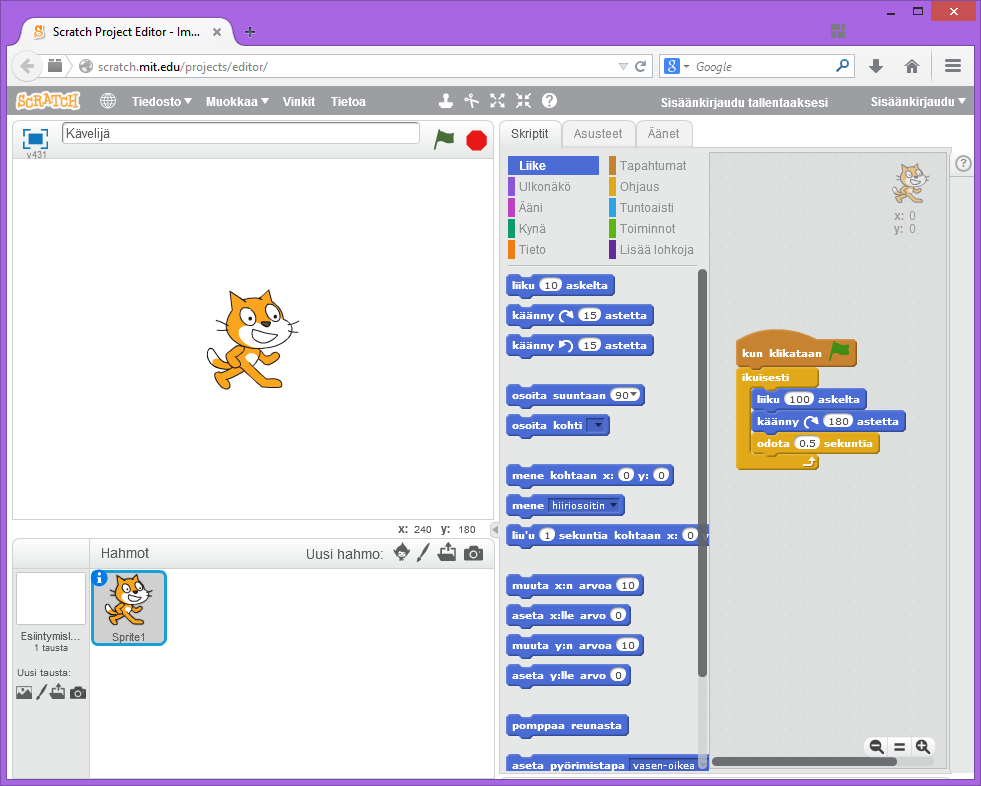
\includegraphics[width=0.5\textwidth]{scratch}
    \caption{Scratch-ohjelmointiympäristö, jossa vasemmassa yläkulmassa suoritusalue ja oikealla ohjelmointialue, jossa lyhyt ohjelmakoodi.}
    \label{img:scratch}
\end{figure}

OPS 2016 -opetussuunnitelman
mukaan peruskoulun luokilla
1 -- 2 on tarkoitus opiskella
vaiheittaisten toimintaohjeiden
antamista.
Luokilla 3 -- 6 on tarkoitus
tutustua ohjelmointiin
graafisten ohjelmointikielten
avulla.
Luokilla 7 -- 9 opiskellaan
hyviä ohjelmointikäytäntöjä
sekä matemaattisten ongelmien
ratkaisemista tietokoneella
\cite{OPS_2016}.
Tämä käytännössä tarkoittaa,
että yläasteella siirrytään
käyttämään tekstipohjaisia
ohjelmointikieliä.

\begin{comment}
Luokat 1-2: Tietokoneella kirjoittaminen, tutustututaan ohjelmistoihin, ikäkaudelle sopiva ohjelmointi. Vaiheittaisten toimintaohjeiden laatiminen matikassa.\\
Luokat 3-6: Opitaan käyttämään ohjelmistoja; toimintalogiikka, mediankäsittely, teknologian toiminta riippuu ihmisten valinnoista, graafiset ohjelmointiympäristöt. Kässässä: harjoitellaan robotiikkaa ja automaatiota.\\
Luokat 7-9: Käsitys ohjelmistojen toimintalogiikasta syvenee. Matikka: algoritmit, ongelmien ratkaiseminen, hyvät ohjelmointikäytännöt, matikkaohjelmat (itse ja valmiit), geometriaohjelmistot. Yksinkertaisen ohjelman ohjelmointi. Kässä: Sulautetut järjestelmät.
\end{comment}

Opetussuunnitelmassa ei
oteta kantaa käytettävään
ohjelmointikieleen.
EppaBasicin on tarkoitus olla
yksi mahdollisuus yläluokilla
käytettäväksi ohjelmointikieleksi.
Myös käyttö alaluokilla on
mahdollista.